\documentclass[a4paper, 12pt]{article}

\usepackage[portuguese]{babel}
\usepackage[utf8]{inputenc}
\usepackage[T1]{fontenc}
\usepackage{amsmath}
\usepackage{url}
\usepackage{amssymb}
\usepackage{booktabs}
\usepackage{tikz}

\usepackage{graphicx}
\usepackage{caption}
\usepackage{subcaption}

\usepackage{algorithm}
\usepackage{algpseudocode}

\graphicspath{{../img/}}

\newcommand{\rom}[1]{\uppercase\expandafter{\romannumeral #1\relax}}

\linespread{1.25}

\begin{document}

\begin{titlepage}
    \centering
    \vspace*{4cm}
    \textbf{\Large{Trabalho \rom{2} de MAC5832: \\ Gradiente Estocástico Descendente, \\
    Modelos de Regressão e Regularização $L_2$}}\\

    \vskip 1cm

    Pedro Henrique Rocha Bruel

    \emph{phrb@ime.usp.br}

    \emph{nUSP: 7143336}

    \vfill
    \normalsize{\emph{DCC - IME\\
    Universidade de São Paulo}\\}
    \normalsize{São Paulo, \today}
\end{titlepage}

\section{Introdução} \label{sec:intro}

Este relatório descreve as implementações realizadas para o Trabalho $2$ da
disciplina \textit{MAC5832}, apresenta análises de acurácia em relação a
diferentes parâmetros e comparações dessas implementações com algoritmos do
pacote \texttt{Scikit Learn}.

Foram implementados um algoritmo para Gradiente Estocástico Descendente, dois
modelos de regressão e um método de regularização, totalizando quatro
combinações de modelos: Regressão Linear, Regressão Linear com Regularização
$L_2$, Regressão Logística e Regressão Logística com Regularização $L_2$.

\subsection{Estrutura de Diretórios}

Os diretórios deste trabalho estão organizados da
seguinte forma:

\paragraph{\texttt{./doc}} Contém os arquivos necessários
para gerar este documento.

\paragraph{\texttt{./src}} Contém o código implementado
para os modelos de regressão e experimentos.

\paragraph{\texttt{./img}} Contém as figuras apresentadas neste relatório.

\section{Gradiente Estocástico Descendente}

O método do \textit{Gradiente Estocástico Descendente} é uma técnica iterativa
para minimização de funções duplamente diferenciáveis. No nosso caso, o método
é aplicado para minimizar o erro de classificação $E_{in}(\textbf{w},
\textbf{X}, \textbf{y})$, onde $\textbf{w}$ é um vetor de pesos, \textbf{X} é
uma matriz de exemplos, ou amostras, e \textbf{y} é um vetor de classificações,
onde cada classificação $\textbf{y}(i)$ corresponde a um exemplo
$\textbf{X}(i)$.

Para encontrar o vetor de pesos $\textbf{w}^{*}$ que minimiza $E_{in}(\cdot)$,
cada iteração do método do Gradiente Estocástico Descendente calcula o
\textit{gradiente} $\nabla{}E_{in}(\cdot)$ e atualiza o vetor atual de pesos.

A técnica do Gradiente Estocástico Descendente pode ser compreendida
intuitivamente como a \lq\lq{}exploração\rq\rq{} de um terreno com diferentes
inclinações e profundidades, utilizando uma bola sujeita à força da gravidade.
O movimento da bola no terreno tenderá a estabilizar-se no ponto do terreno com
menor profundidade, mas o local inicial terá bastante impacto no local final.
Formas de atenuar esse problema incluem utilizar várias bolas ao mesmo tempo,
ou bolas com \lq\lq{}coeficientes de atrito\rq\rq{} diferentes.

\subsection{Algoritmo}

A implementação da técnica do Gradiente Estocástico Descendente deste trabalho
foi feita na linguagem \texttt{Python 3.5.1} e está descrita em pseudocódigo no
Algoritmo \ref{alg:GSD}. O resto desta Seção descreve a implementação em
detalhes.

\subsubsection{Parâmetros}

A implementação foi feita de forma \textit{modular}, permitindo que funções
para o cálculo do gradiente e da taxa de aprendizagem fossem passadas como
parâmetro. Esta Seção descreve os parâmetros para o algoritmo implementado.

\paragraph{Taxa de Aprendizagem inicial ($\alpha^{\prime}$):}

Em todos os experimentos deste trabalho utilizei a seguinte função
para o cálculo da taxa de aprendizagem $\alpha(i)$, onde $i$ é o número da
iteração atual do algoritmo, e $\alpha^{\prime}$ é a taxa de aprendizagem
inicial:

\begin{align*}
    \alpha(i) = \frac{\alpha^{\prime}}{1 + log_{2}i}
\end{align*}

Seguindo a metáfora para a compreensão intuitiva da técnica, a ideia é
modificar o \lq\lq{}coeficiente de atrito\rq\rq{}, isto é, a taxa de
aprendizagem, para que em iterações inicias sejam permitidas variações maiores
no vetor de pesos, e posteriomente na execução do algoritmo, apenas
\lq\lq{}saltos\rq\rq{} menores.

\paragraph{Função do Gradiente ($\nabla{}E_{in}(\cdot)$):}

A expressão para o cálculo do gradiente será diferente, de acordo com o modelo
de regressão que utilizarmos em conjunto com a técnica de Gradiente Estocástico
Descendente. As expressões para cálculo do gradiente dos quatros modelos de
regressão implementados neste trabalho estão descritas na Seção \ref{sec:regr}.

A implementação de todas as funções de gradiente recebe como entrada um vetor
de pesos \textbf{w}, e um subconjunto dos exemplos em \textbf{X}, junto com
suas classificações em \textbf{y} correspondentes. A saída dessas funções é o
gradiente calculado de acordo com o modelo de regressão correspondente.

\paragraph{Número de Iterações ($I$):}

É o número de iterações realizadas antes de se devolver o vetor final de pesos
$\textbf{w}(I)$.

\paragraph{Vetor Inicial de Pesos ($\textbf{w}(0)$):}

Deve ter o mesmo número de elementos em cada exemplo de \textbf{X}.
É inicializado com zeros.

\paragraph{Matriz de Exemplos ($\textbf{X}$):}

Contém os exemplos para teste em suas linhas.

\paragraph{Vetor de Classificações ($\textbf{y}$):}

A posição $\textbf{y}(i)$ contém a classificação
do exemplo $\textbf{X}(i)$.

\paragraph{Tamanho do \textit{Batch} ($\sigma$):}

Determina o tamanho do subconjunto de exemplos que será utilizado em cada
iteração. O tamanho do conjunto de dados não permitiu que os gradientes
fossem calculados usando todo o conjunto de uma só vez. Para contornar
isso utilizei um parâmetro que determina a \textit{porcentagem} do
conjunto que será utilizada nas iterações.

A cada iteração são calculados os conjuntos $\textbf{X}[\sigma]$ e
$\textbf{y}[\sigma]$, que contém $m$  elementos escolhidos \textit{ao acaso},
onde $m = |\textbf{X}| \cdot \sigma$, e $|\textbf{X}|$ é o número total de
exemplos.  Dessa forma é possível usar todo o conjunto de dados sem pagar o
custo dos produtos escalares de matrizes enormes.

\subsubsection{Saída}

\paragraph{Vetor Final de Pesos ($\textbf{w}(I)$):}

Contém um peso para cada característica dos exemplos de teste
em \textbf{X}. É usado posteriormente para fazer as predições
de classificação.

\begin{algorithm}[htpb]
    \caption{Gradiente Estocástico Descendente \\ com Taxa de Aprendizagem Variante}
    \label{alg:GSD}
    \begin{algorithmic}[1]
        \Statex \item[\textbf{Input:}]
        \Statex $\nabla{}E_{in}(\cdot)$ \Comment Função para cálculo do Gradiente
        \Statex $I$ \Comment Número de Iterações
        \Statex $\sigma$ \Comment Tamanho do \textit{batch}
        \Statex $\alpha^{\prime}$ \Comment Taxa de Aprendizagem inicial
        \Statex $\textbf{w}(0)$ \Comment Vetor inicial de pesos
        \Statex $\textbf{X}$ \Comment Matriz de exemplos
        \Statex $\textbf{y}$ \Comment Vetor de classificações
        \Statex \item[\textbf{Output:}]
        \Statex $\textbf{w}(I)$ \Comment Vetor final de pesos
        \Statex
        \For{$i = 1, 2, \dots, I$}
        \State Calcule $\textbf{g}_i = \nabla{}E_{in}(\textbf{w}(i),\: \textbf{X}[\sigma],\: \textbf{y}[\sigma])$
        \State Calcule $\alpha(i) = \frac{\alpha^{\prime}}{1 + log_{2}i}$
        \State Calcule $\textbf{w}(i) = \textbf{w}(i -1) - \alpha{}\textbf{g}_i$
        \EndFor
        \State \Return $\textbf{w}(I)$
    \end{algorithmic}
\end{algorithm}


\section{Modelos de Regressão} \label{sec:regr}

Esta Seção apresenta as expressões para os modelos de regressão implementados
em \texttt{Python 3.5.1}, usando o módulo \texttt{numpy}.

\subsection{Regressão Linear}

A ideia deste modelo é separar, se possível, o conjunto de dados com um plano
de dimensão $|\textbf{w}|$, isto é, de dimensão igual ao número de
características dos exemplos. Além disso, a soma dos quadrados das distâncias
entre os exemplos e o plano deve ser minimizada.
A hipótese no caso da Regressão Linear é dada por:

\begin{align*}
    h(\textbf{X}(i),\textbf{w}) = \textbf{w}^{T}\textbf{X}(i)
\end{align*}


\paragraph{Expressão para $E_{in}(\cdot)$}

\begin{align*}
    E_{in}(\textbf{w}, \textbf{X}, \textbf{y}) = \frac{1}{|\textbf{X}|} \|\textbf{Xw} - \textbf{y}\|^{2}
\end{align*}

Onde $|\textbf{X}|$ é o número total de exemplos.

\paragraph{Expressão para $\nabla{}E_{in}(\cdot)$}

\begin{align*}
    \nabla{}E_{in}(\textbf{w}, \textbf{X}, \textbf{y}) = \frac{2}{|\textbf{X}|} (\textbf{X}^{T}\textbf{Xw} - \textbf{X}^{T}\textbf{y})
\end{align*}

\subsection{Regressão Logística}

A ideia deste algoritmo é considerar a \textit{probabilidade} de classificação
dos exemplos, e não apenas um valor binário. A hipótese no caso da Regressão
Logística é dada por:

\begin{align*}
    h(\textbf{X}(i),\textbf{w}) = \theta(\textbf{w}^{T}\textbf{X}(i))
\end{align*}

Onde a função $\theta(\cdot)$ produz valores \textit{entre} $0$ e $1$, e é
chamada de \textit{função logística}:

\begin{align*}
    \theta(s) = \frac{e^{s}}{1 + e^{s}}
\end{align*}

\paragraph{Expressão para $E_{in}(\cdot)$}

\begin{align*}
    E_{in}(\textbf{w}, \textbf{X}, \textbf{y}) = \frac{1}{|\textbf{X}|} \sum^{|\textbf{X}|}_{i=1}{ln(1 + e^{-\textbf{y}(i)\textbf{w}^{T}\textbf{X}(i)})}
\end{align*}

\paragraph{Expressão para $\nabla{}E_{in}(\cdot)$}

\begin{align*}
    \nabla{}E_{in}(\textbf{w}, \textbf{X}, \textbf{y}) = -\frac{1}{|\textbf{X}|} \sum^{|\textbf{X}|}_{i=1}{\frac{\textbf{y}(i)\textbf{X}(i)}{1 + e^{\textbf{y}(i)\textbf{w}^{T}\textbf{X}(i)}}}
\end{align*}

\subsection{Regressão Linear com Regularização $L_2$}

A \textit{Regularização} é uma estratégia para \lq\lq{}combater\rq\rq{} a
tendência que os modelos de regularização apresentam de ajustar-se demais ao
conjunto de dados de treino, num processo chamado de \textit{overfitting}.

Utilizamos neste trabalho o método para regularização introduzido por
\textit{Andrey Tikhonov}, conhecido como \textit{Ridge Regression}.
Na discussão do livro-texto, esse método de regressão é apresentado
como a adição de uma limitação, ou \textit{constraint}, à otimização
do $E_{in}$ de um dado modelo de regressão.

No caso da \textit{Regularização $L_2$} essa limitação é representada pelo termo:

\begin{align*}
    E_{in}(\textbf{w}) = -\lambda\|\textbf{w}\|^{2}
\end{align*}

Onde $\lambda > 0$ é um parâmetro a ser escolhido. O gradiente do termo
de regularização é dado por:

\begin{align*}
    \nabla{}E_{in}(\textbf{w}) = -2\lambda{}\textbf{w}
\end{align*}

Adicionando o termo de regularização ao modelo de Regressão Linear, temos:

\paragraph{Expressão para $E_{in}(\cdot)$}

\begin{align*}
    E_{in}(\textbf{w}, \textbf{X}, \textbf{y}) = \frac{1}{|\textbf{X}|} \|\textbf{Xw} - \textbf{y}\|^{2} - \lambda\|\textbf{w}\|^{2}
\end{align*}

\paragraph{Expressão para $\nabla{}E_{in}(\cdot)$}

Considerando a propriedade de $\nabla$:

\begin{align*}
    \nabla(f + g) = \nabla(f) + \nabla(g)
\end{align*}

E usando a expressão para $\nabla{}E_{in}(\cdot)$ da Regressão Linear, temos:

\begin{align*}
    \nabla{}E_{in}(\textbf{w}, \textbf{X}, \textbf{y}) = \frac{2}{|\textbf{X}|} (\textbf{X}^{T}\textbf{Xw} - \textbf{X}^{T}\textbf{y}) - 2\lambda\textbf{w}
\end{align*}

\subsection{Regressão Logística com Regularização $L_2$}

Adicionando o termo de regularização ao modelo de Regressão Logística, temos:

\paragraph{Expressão para $E_{in}(\cdot)$}

\begin{align*}
    E_{in}(\textbf{w}, \textbf{X}, \textbf{y}) = \frac{1}{|\textbf{X}|} \sum^{|\textbf{X}|}_{i=1}{ln(1 + e^{-\textbf{y}(i)\textbf{w}^{T}\textbf{X}(i)})} - \lambda\|\textbf{w}\|^{2}
\end{align*}

\paragraph{Expressão para $\nabla{}E_{in}(\cdot)$}

\begin{align*}
    \nabla{}E_{in}(\textbf{w}, \textbf{X}, \textbf{y}) = -\frac{1}{|\textbf{X}|} \sum^{|\textbf{X}|}_{i=1}{\frac{\textbf{y}(i)\textbf{X}(i)}{1 + e^{\textbf{y}(i)\textbf{w}^{T}\textbf{X}(i)}}} - 2\lambda\textbf{w}
\end{align*}

\subsection{Modelos do \texttt{Scikit Learn}}

Utilizei as implementações para Regressão Linear, Regressão Linear com
Regularização $L_2$ e Regressão Logística com Regularização $L_2$ disponíveis
no módulo \texttt{sklearn.linear\_model} do pacote \texttt{Scikit Learn}.  Não
utilizei o método de Regressão Logística sem Regularização.

\section{Resultados}

Esta Seção apresenta os resultados obtidos medindo a acurácia dos modelos de
regressão implementados para o trabalho. O desempenho dos modelos foi avaliado
usando o conjunto de dados disponibilizado pelo monitor da disciplina. Neste
trabalho, a acurácia é a porcentagem de exemplos no conjunto de testes que
foram classificados corretamente.

O objetivo dessas avaliações de desempenho é estudar como cada modelo de
regressão e regularização se comporta quanto à acurácia em relação a seus
parâmetros. Busquei encontrar os valores ideais dos parâmetros $I$ (Número de
Iterações), $\sigma$ (Tamanho do \textit{Batch}), $\lambda$ (Parâmetro de
Regularização) e $\alpha$ (Taxa de Aprendizagem) para cada modelo de regressão
e regularização.

Os pontos de todos os gráficos apresentados nessa Seção foram obtidos
calculando a média de 10 execuções do respectivo modelo com os parâmetros
em questão. Cada ponto também apresenta o erro padrão calculado à partir
das 10 medições.

\newpage
\subsection{Acurácia vs. Iterações}

Como era de se esperar, a acurácia do algoritmo para o Gradiente
Estocástico Descendente aumenta com o Número de Iterações. Note
que o aumento da acurácia diminui depois de cerca de $15000$ iterações.
Também é interessante notar que o erro padrão das amostras para o modelo de
Regressão Linear com Regularização $L_2$ é maior que o das amostras de outros
modelos. Não sei explicar o porquê.

\begin{figure}[htpb]
    \centering
    \begin{subfigure}[htpb]{0.45\textwidth}
        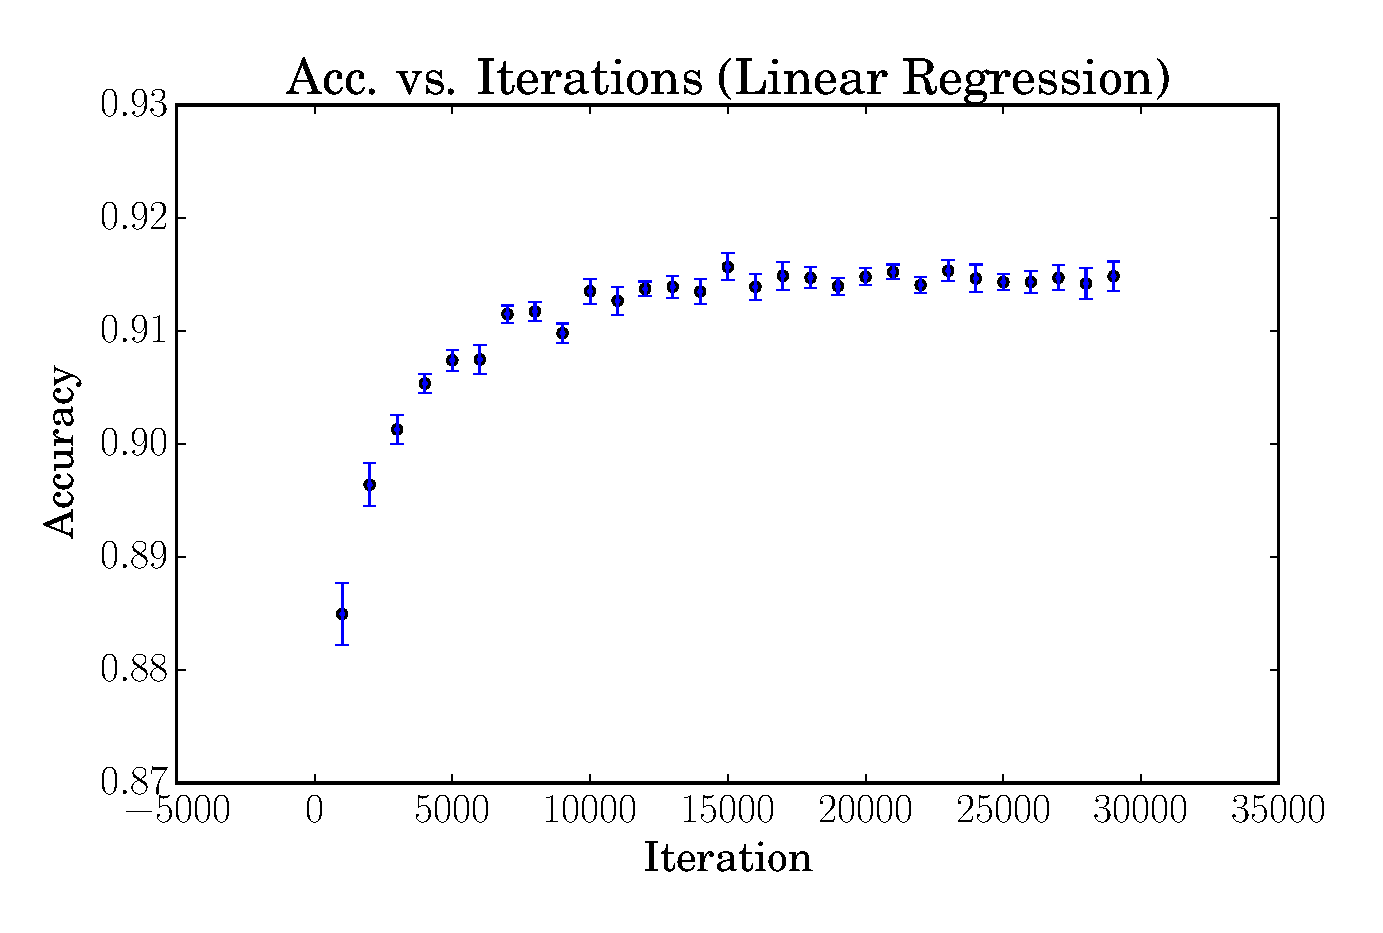
\includegraphics[width=\textwidth]{acc_vs_iterations_linreg}
        \caption{}
        \label{fig:it_linreg}
    \end{subfigure}
    %add desired spacing between images, e. g. ~, \quad, \qquad, \hfill etc.
    %(or a blank line to force the subfigure onto a new line)
    \begin{subfigure}[htpb]{0.45\textwidth}
        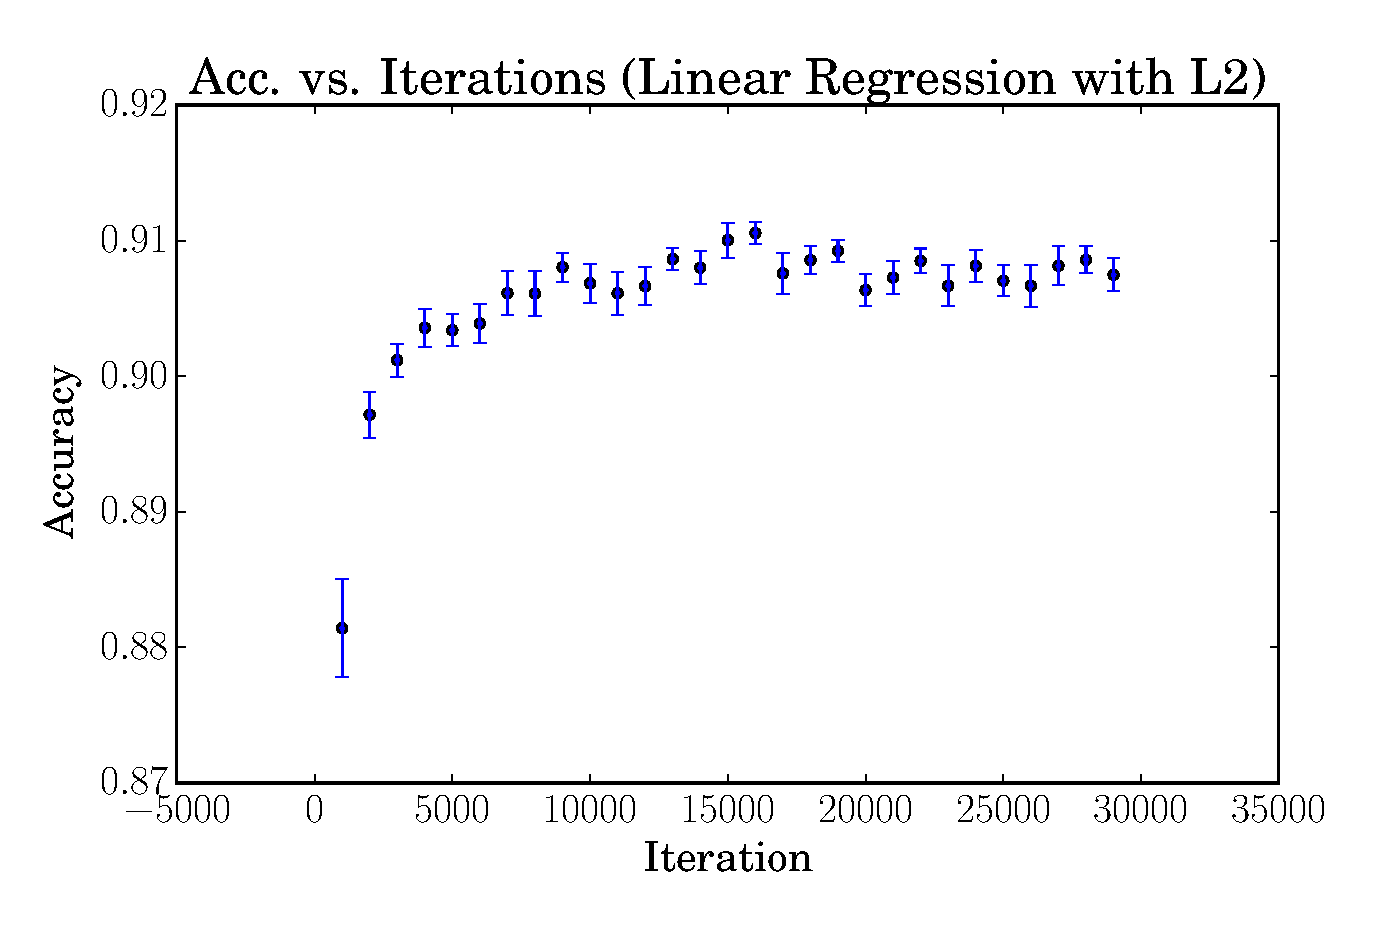
\includegraphics[width=\textwidth]{acc_vs_iterations_linregL2}
        \caption{}
        \label{fig:it_linregL2}
    \end{subfigure}
    \hfill %add desired spacing between images, e. g. ~, \quad, \qquad, \hfill etc.
    %(or a blank line to force the subfigure onto a new line)
    \begin{subfigure}[htpb]{0.45\textwidth}
        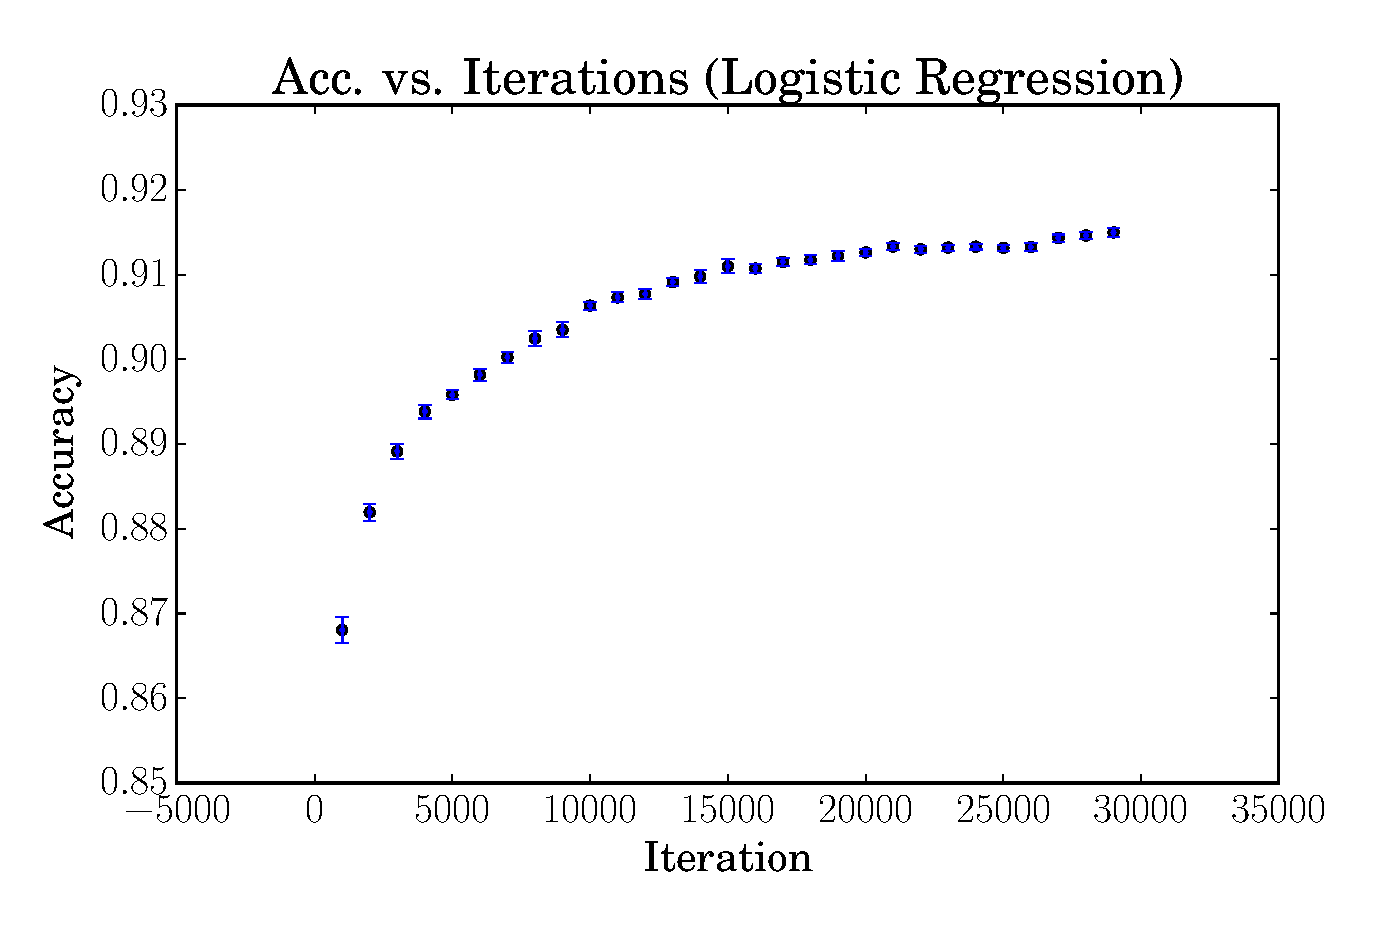
\includegraphics[width=\textwidth]{acc_vs_iterations_logreg}
        \caption{}
        \label{fig:it_logreg}
    \end{subfigure}
    %add desired spacing between images, e. g. ~, \quad, \qquad, \hfill etc.
    %(or a blank line to force the subfigure onto a new line)
    \begin{subfigure}[htpb]{0.45\textwidth}
        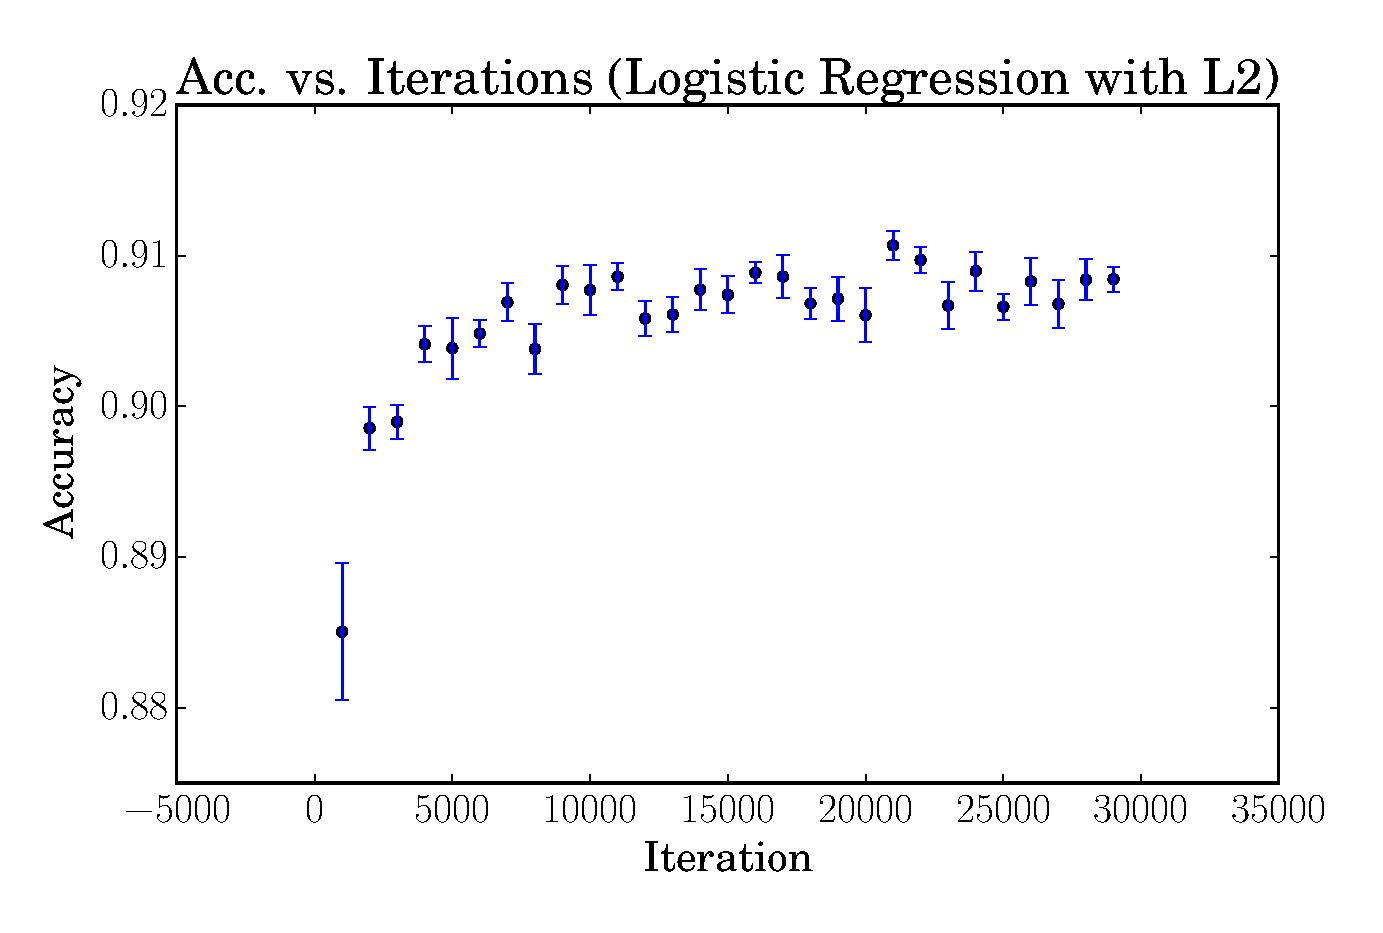
\includegraphics[width=\textwidth]{acc_vs_iterations_logregL2}
        \caption{}
        \label{fig:it_logregL2}
    \end{subfigure}
    \caption{Acurácia vs. Número de Iterações ($I$) do Gradiente Estocástico
    Descendente, com parâmetros fixos: $\lambda=0.0051$, $\alpha=0.5$,
    $\sigma=10^{-3}$}\label{fig:it}
\end{figure}

\newpage
\subsection{Acurácia vs. Taxa de Aprendizagem}

Os resultados para a Regressão Linear e a Regressão Linear com Regularização
$L_2$ apresentaram acurácia de $0\%$ para $\alpha > 2^{0}$ por conta de erros
de \textit{overflow}. Uma possível maneira de resolver esse problema seria
normalizar o vetor de pesos. Não experimentei essa solução pois os pontos
válidos para esses modelos mostram que a acurácia começa a diminuir para
$\alpha > 2^{-1}$. Note que cada algoritmo tem um valor preferível de $\alpha$.

\begin{figure}[htpb]
    \centering
    \begin{subfigure}[htpb]{0.45\textwidth}
        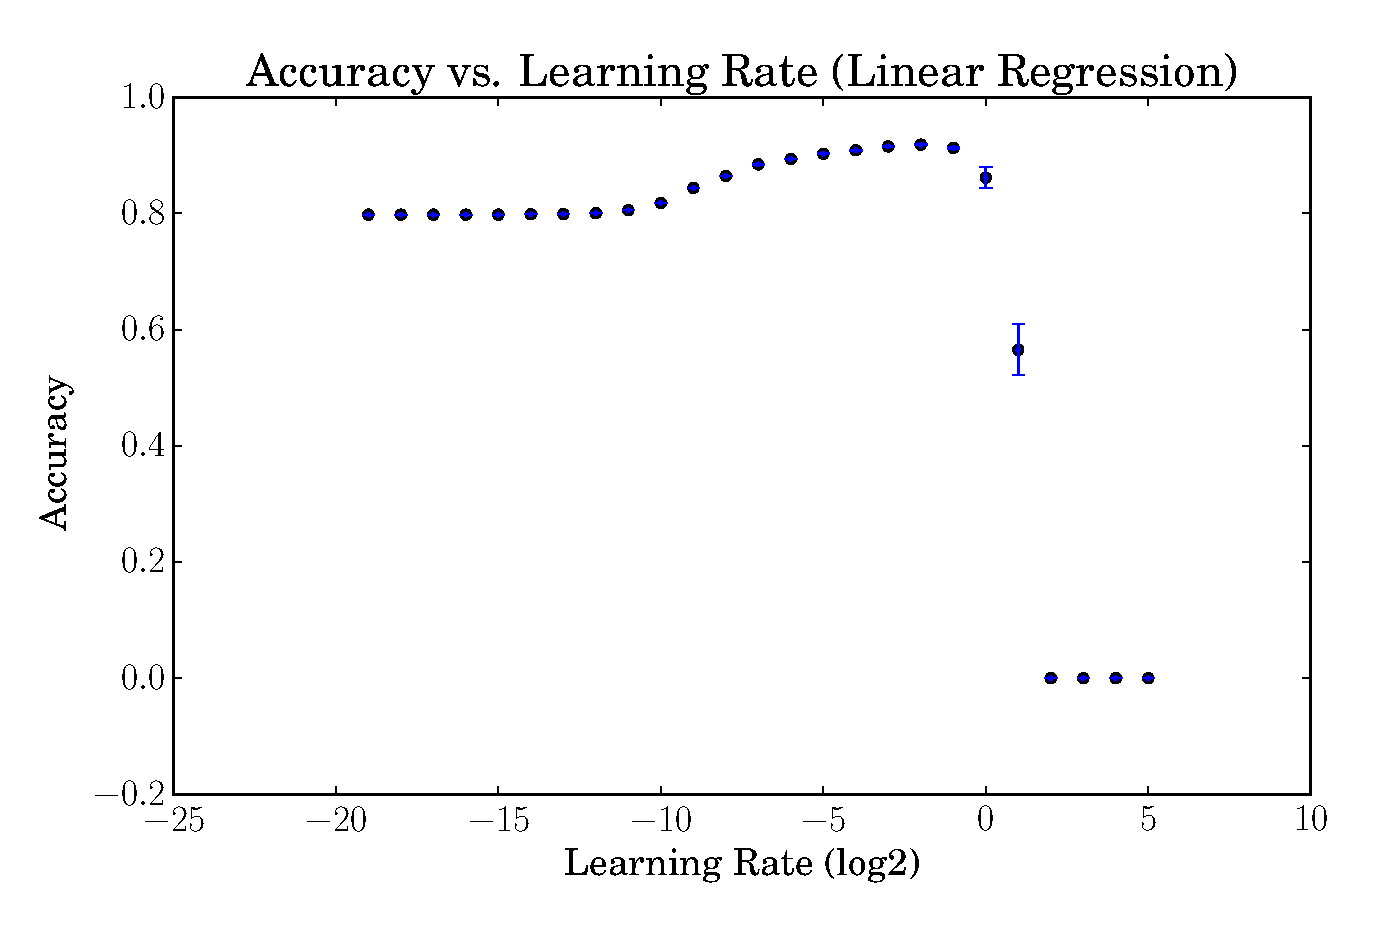
\includegraphics[width=\textwidth]{acc_vs_rate_linreg}
        \caption{}
        \label{fig:rate_lingreg}
    \end{subfigure}
    %add desired spacing between images, e. g. ~, \quad, \qquad, \hfill etc.
    %(or a blank line to force the subfigure onto a new line)
    \begin{subfigure}[htpb]{0.45\textwidth}
        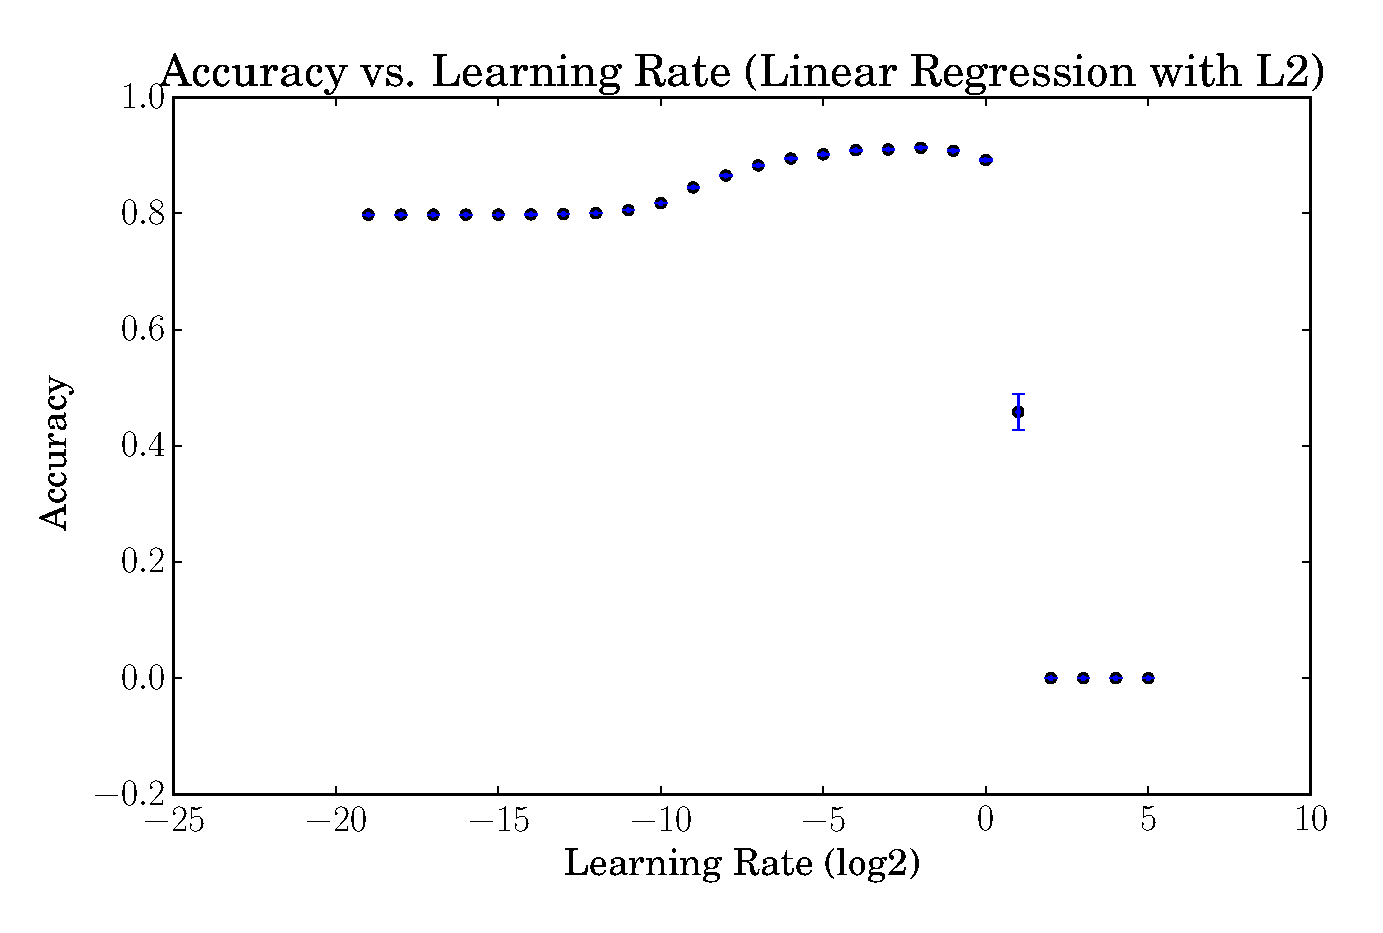
\includegraphics[width=\textwidth]{acc_vs_rate_linregL2}
        \caption{}
        \label{fig:rate_linregL2}
    \end{subfigure}
    \hfill %add desired spacing between images, e. g. ~, \quad, \qquad, \hfill etc.
    %(or a blank line to force the subfigure onto a new line)
    \begin{subfigure}[htpb]{0.45\textwidth}
        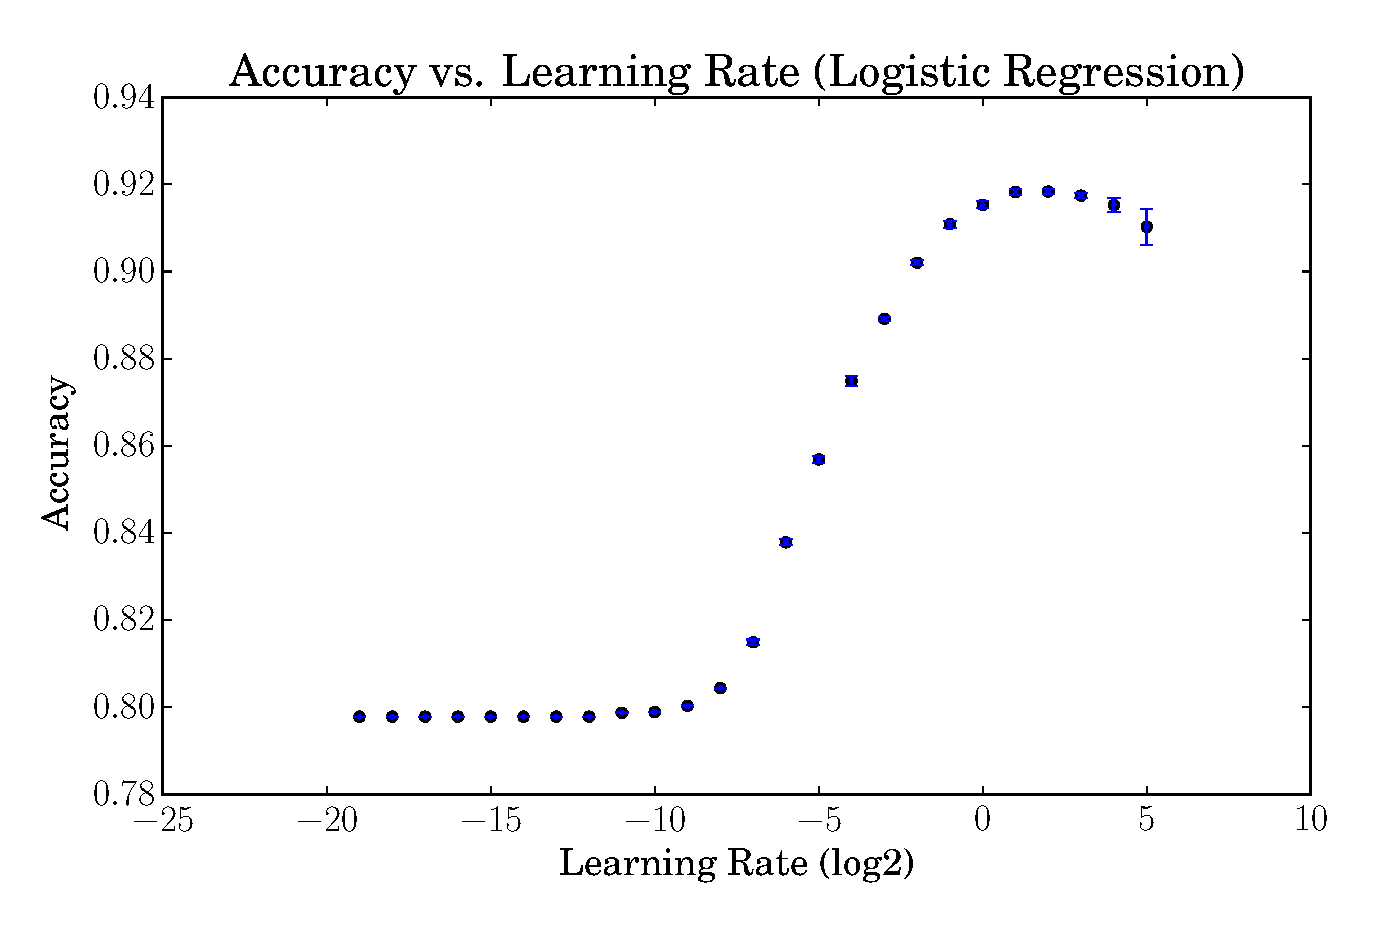
\includegraphics[width=\textwidth]{acc_vs_rate_logreg}
        \caption{}
        \label{fig:rate_logreg}
    \end{subfigure}
    %add desired spacing between images, e. g. ~, \quad, \qquad, \hfill etc.
    %(or a blank line to force the subfigure onto a new line)
    \begin{subfigure}[htpb]{0.45\textwidth}
        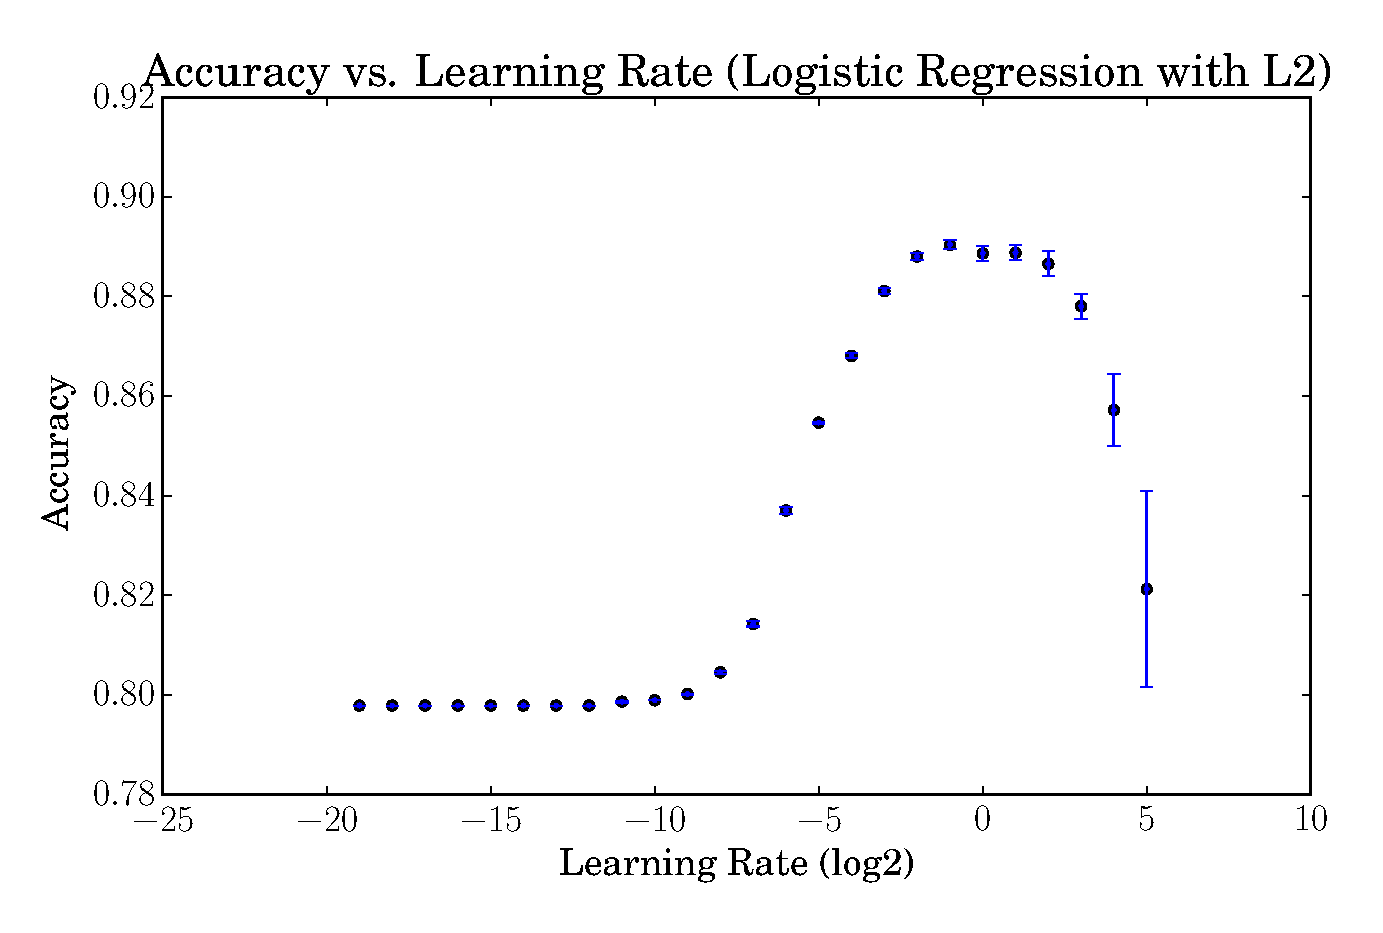
\includegraphics[width=\textwidth]{acc_vs_rate_logregL2}
        \caption{}
        \label{fig:rate_logregL2}
    \end{subfigure}
    \caption{Acurácia vs. Taxa de Aprendizagem ($\alpha$), com parâmetros
    fixos: $\lambda=0.0051$, $I=15000$, $\sigma=10^{-3}$}\label{fig:rate}
\end{figure}

\newpage
\subsection{Acurácia vs. Tamanho do \textit{Batch}}

Novamente, quanto maior a porcentagem $\sigma$ de exemplos do conjunto usados
em cada iteração, maior a acurácia do modelo. É necessário balancear a acurácia
com a capacidade computacional, pois a duração de uma iteração é proporcional a
$\sigma$. Note que o erro padrão é inversamente proporcional a $\sigma$, pois
com mais exemplos usados a variabilidade fica menor.

\begin{figure}[htpb]
    \centering
    \begin{subfigure}[htpb]{0.45\textwidth}
        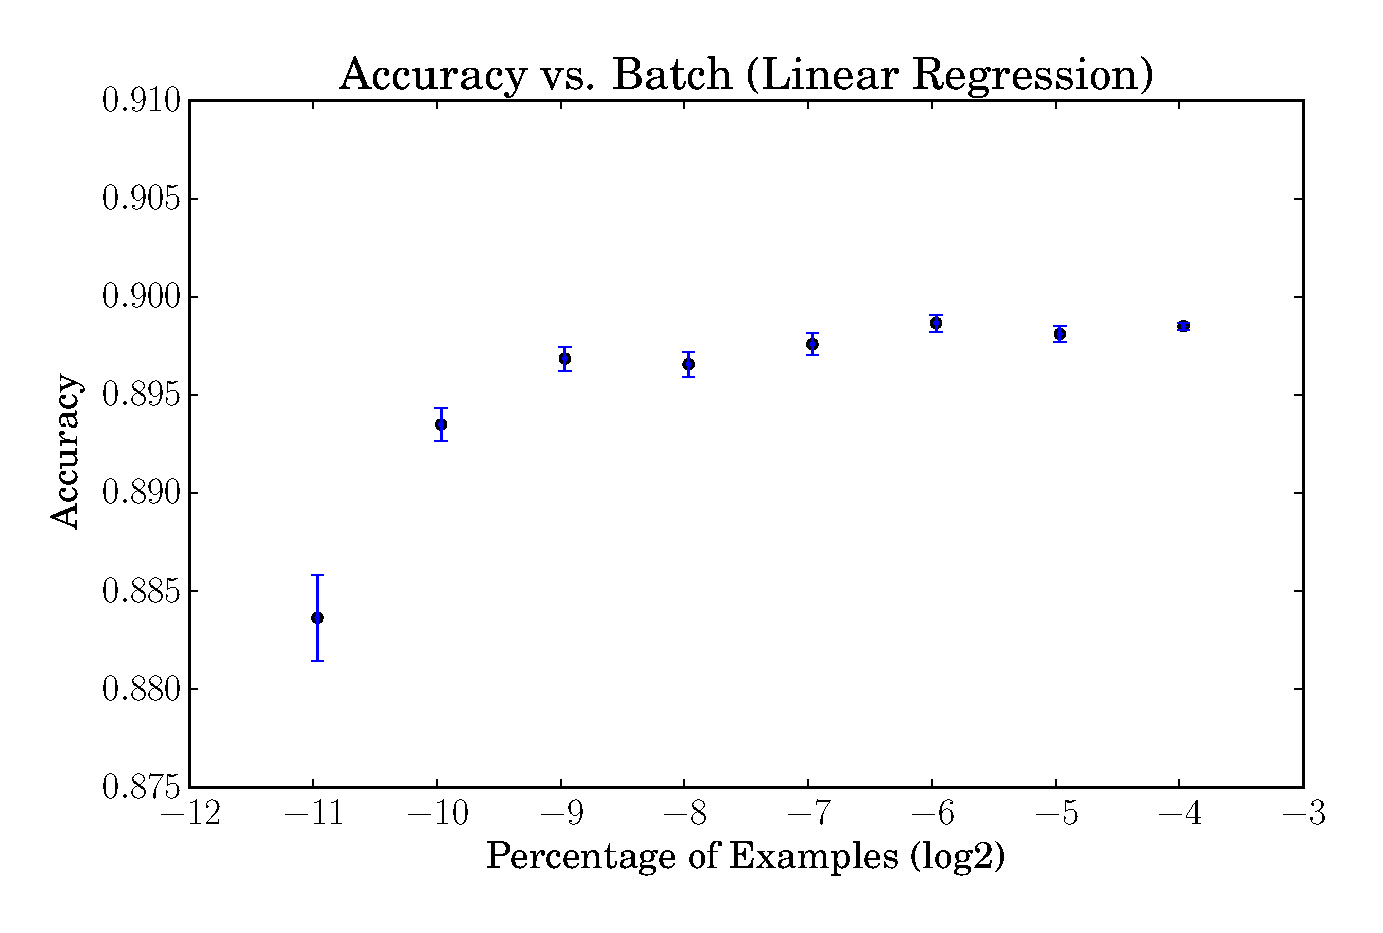
\includegraphics[width=\textwidth]{acc_vs_batchp_linreg}
        \caption{}
        \label{fig:batch_linreg}
    \end{subfigure}
    %add desired spacing between images, e. g. ~, \quad, \qquad, \hfill etc.
    %(or a blank line to force the subfigure onto a new line)
    \begin{subfigure}[htpb]{0.45\textwidth}
        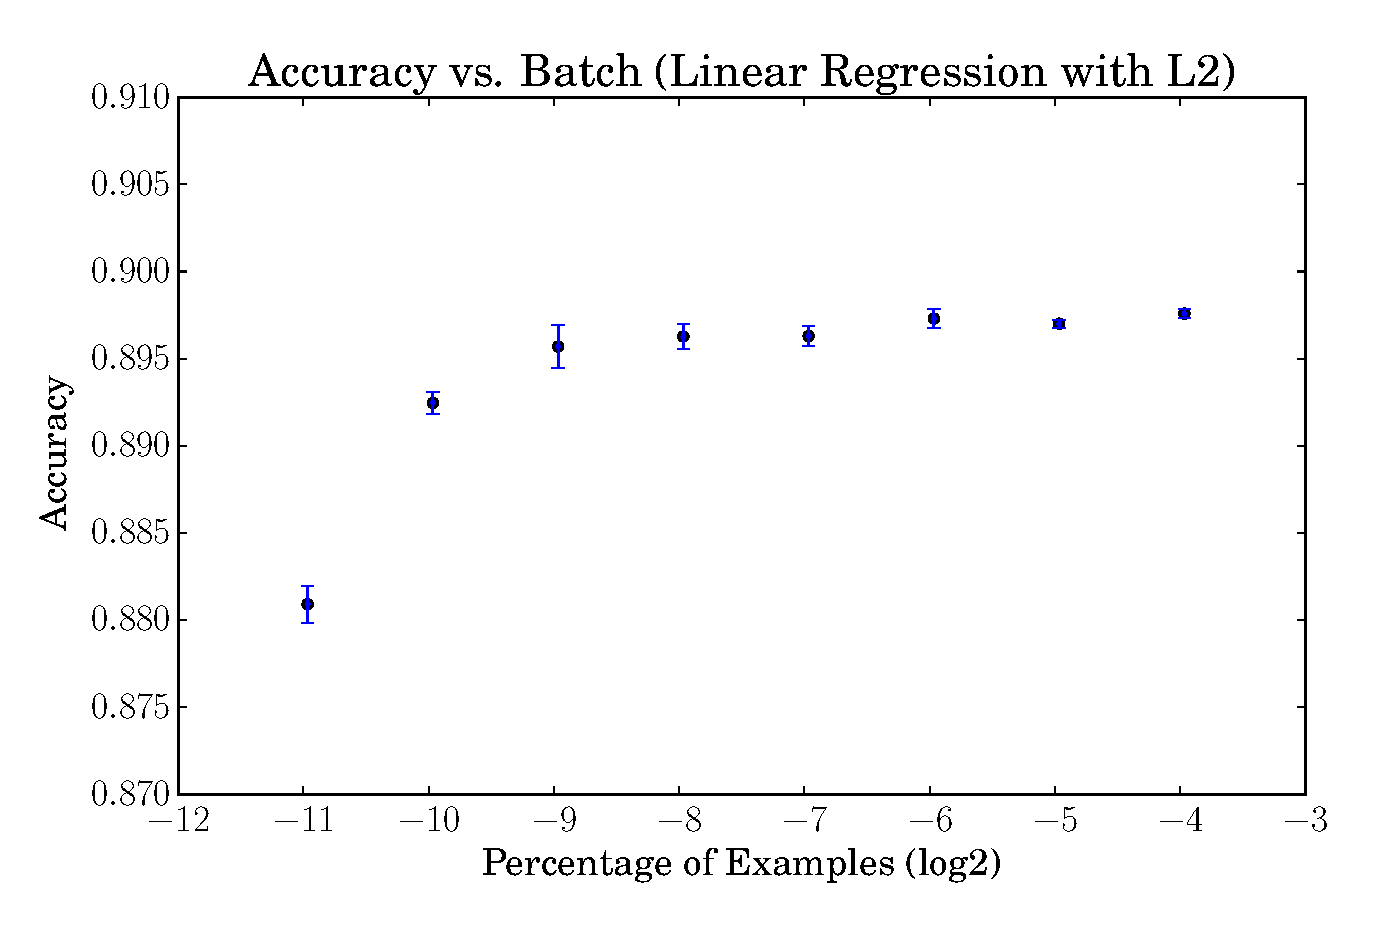
\includegraphics[width=\textwidth]{acc_vs_batchp_linregL2}
        \caption{}
        \label{fig:batch_linregL2}
    \end{subfigure}
    \hfill %add desired spacing between images, e. g. ~, \quad, \qquad, \hfill etc.
    %(or a blank line to force the subfigure onto a new line)
    \begin{subfigure}[htpb]{0.45\textwidth}
        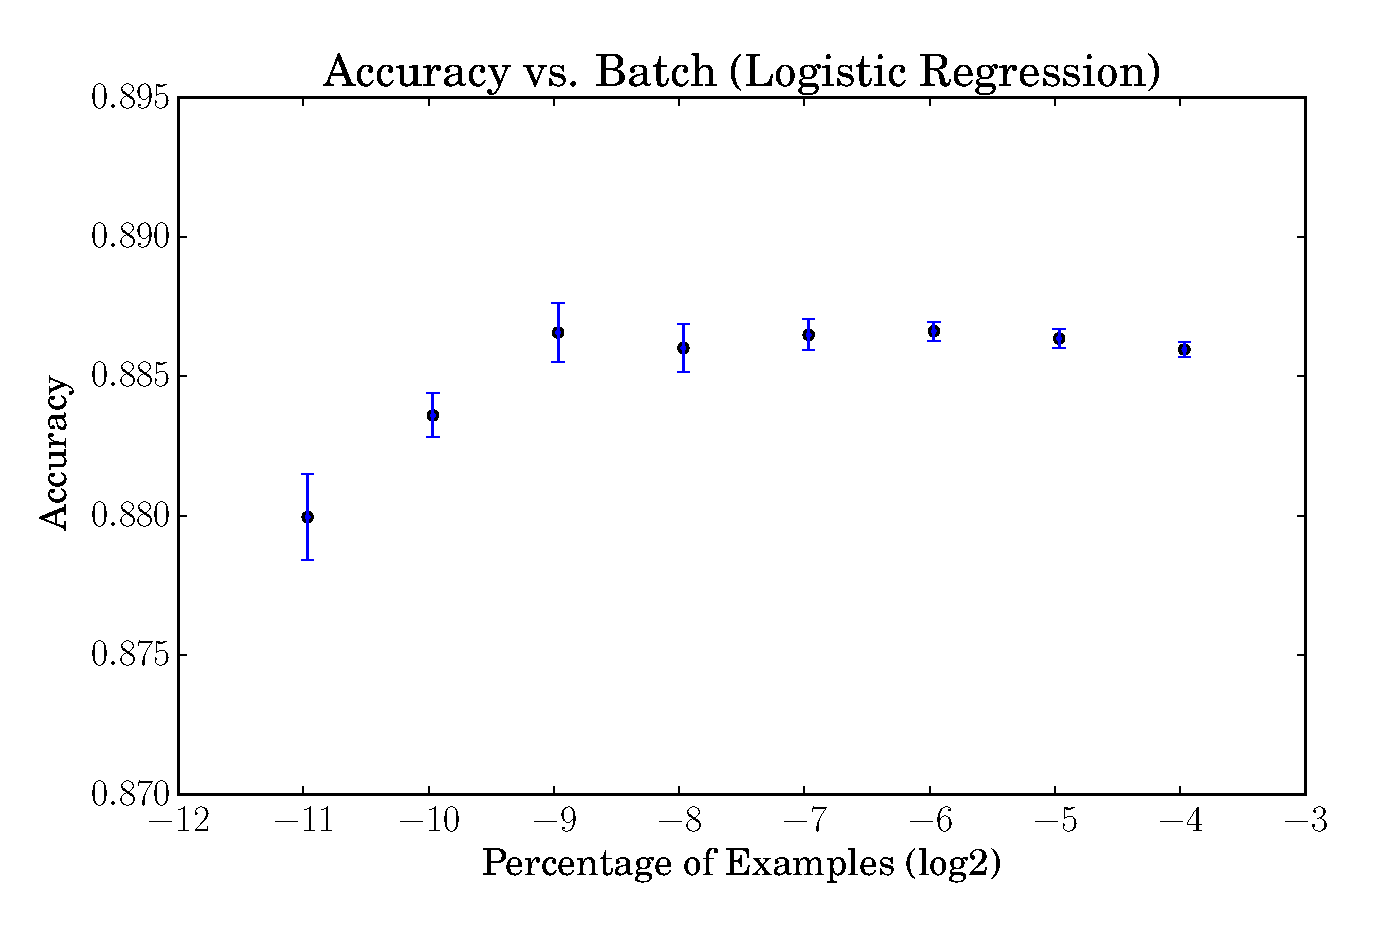
\includegraphics[width=\textwidth]{acc_vs_batchp_logreg}
        \caption{}
        \label{fig:batch_logreg}
    \end{subfigure}
    %add desired spacing between images, e. g. ~, \quad, \qquad, \hfill etc.
    %(or a blank line to force the subfigure onto a new line)
    \begin{subfigure}[htpb]{0.45\textwidth}
        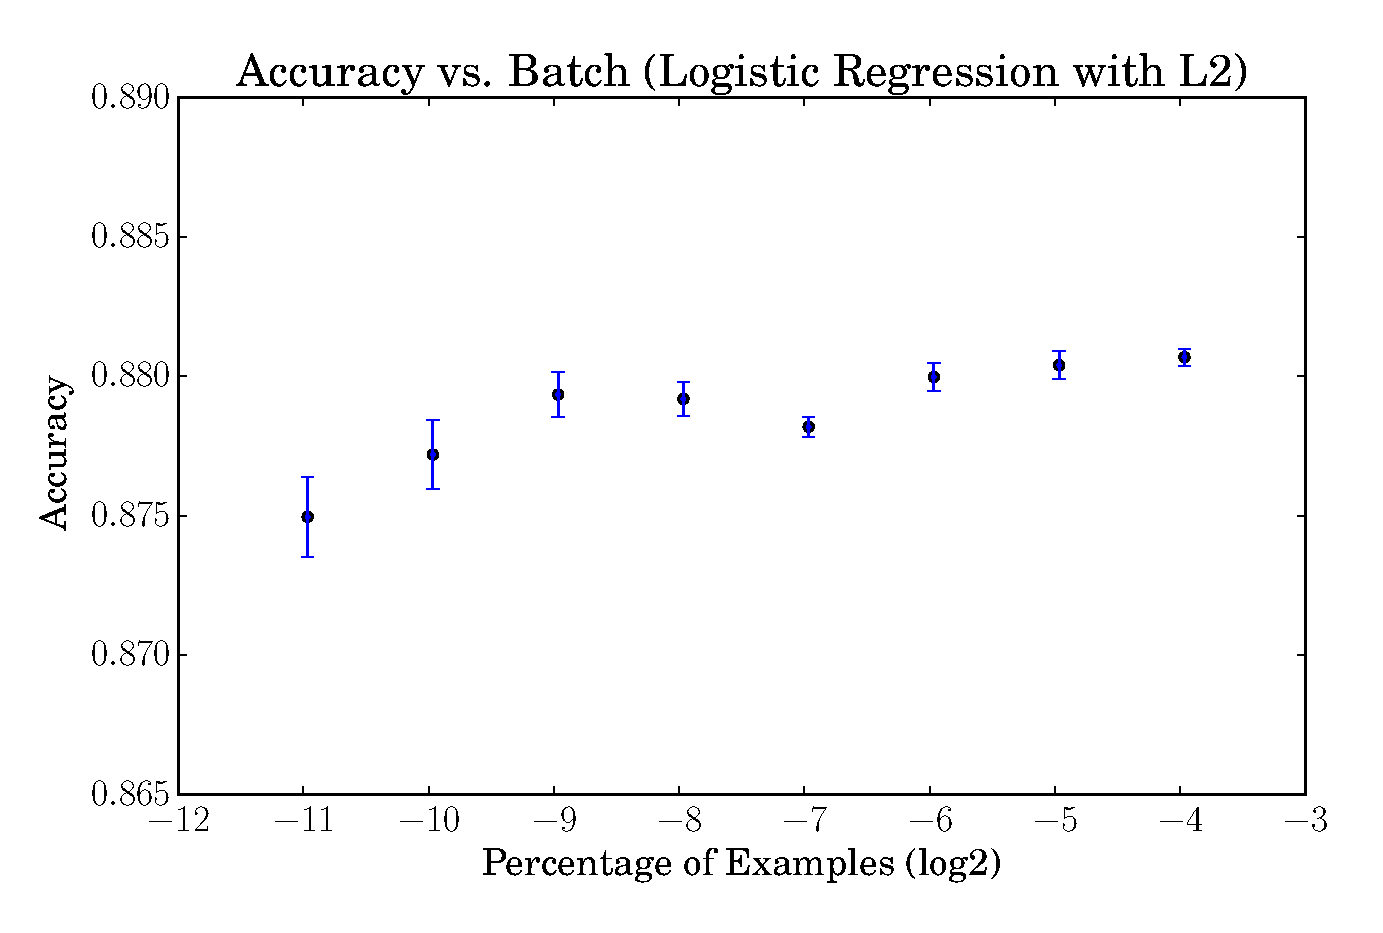
\includegraphics[width=\textwidth]{acc_vs_batchp_logregL2}
        \caption{}
        \label{fig:batch_logregL2}
    \end{subfigure}
    \caption{Acurácia vs. Tamanho do \textit{Batch} ($\sigma$), com
    parâmetros fixos: $\lambda=0.0051$, $I=500$, $\alpha=0.5$}\label{fig:batch}
\end{figure}

\newpage
\subsection{Acurácia vs. $\lambda$}

A acurácia dos modelos em relação a $\lambda$ se comporta de forma distinta
para os dois modelos com regularização implementados. O modelo de Regressão
Linear com Regularização $L_2$ apresenta maior acurácia para $2^{-5} < \lambda
< 2^{0}$, e o modelo de Regressão Logística com Regularização $L_2$ apresenta
melhor acurácia para $\lambda < 2^{-5}$. Alguns valores de $\lambda$ também
resultaram em \textit{overflow}, mas também decidi não implementar
normalizações por que a acurácia pareceu aumentar na outra direção de variação
do parâmetro.

\begin{figure}[htpb]
    \centering
    \begin{subfigure}[htpb]{0.45\textwidth}
        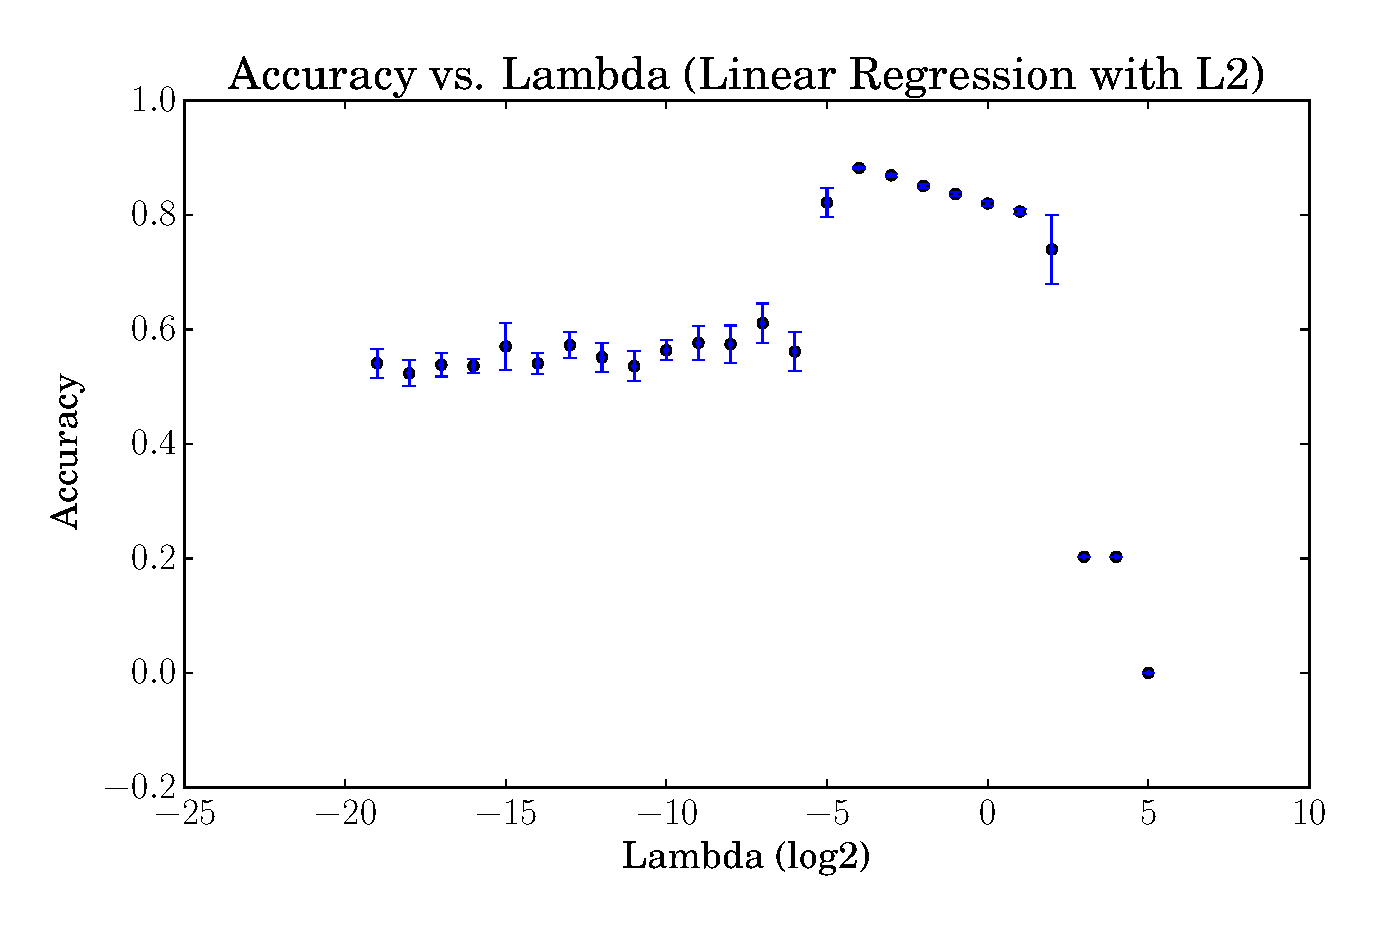
\includegraphics[width=\textwidth]{acc_vs_lambda_linregL2}
        \caption{}
        \label{fig:lambda_linregL2}
    \end{subfigure}
    %add desired spacing between images, e. g. ~, \quad, \qquad, \hfill etc.
    %(or a blank line to force the subfigure onto a new line)
    \begin{subfigure}[htpb]{0.45\textwidth}
        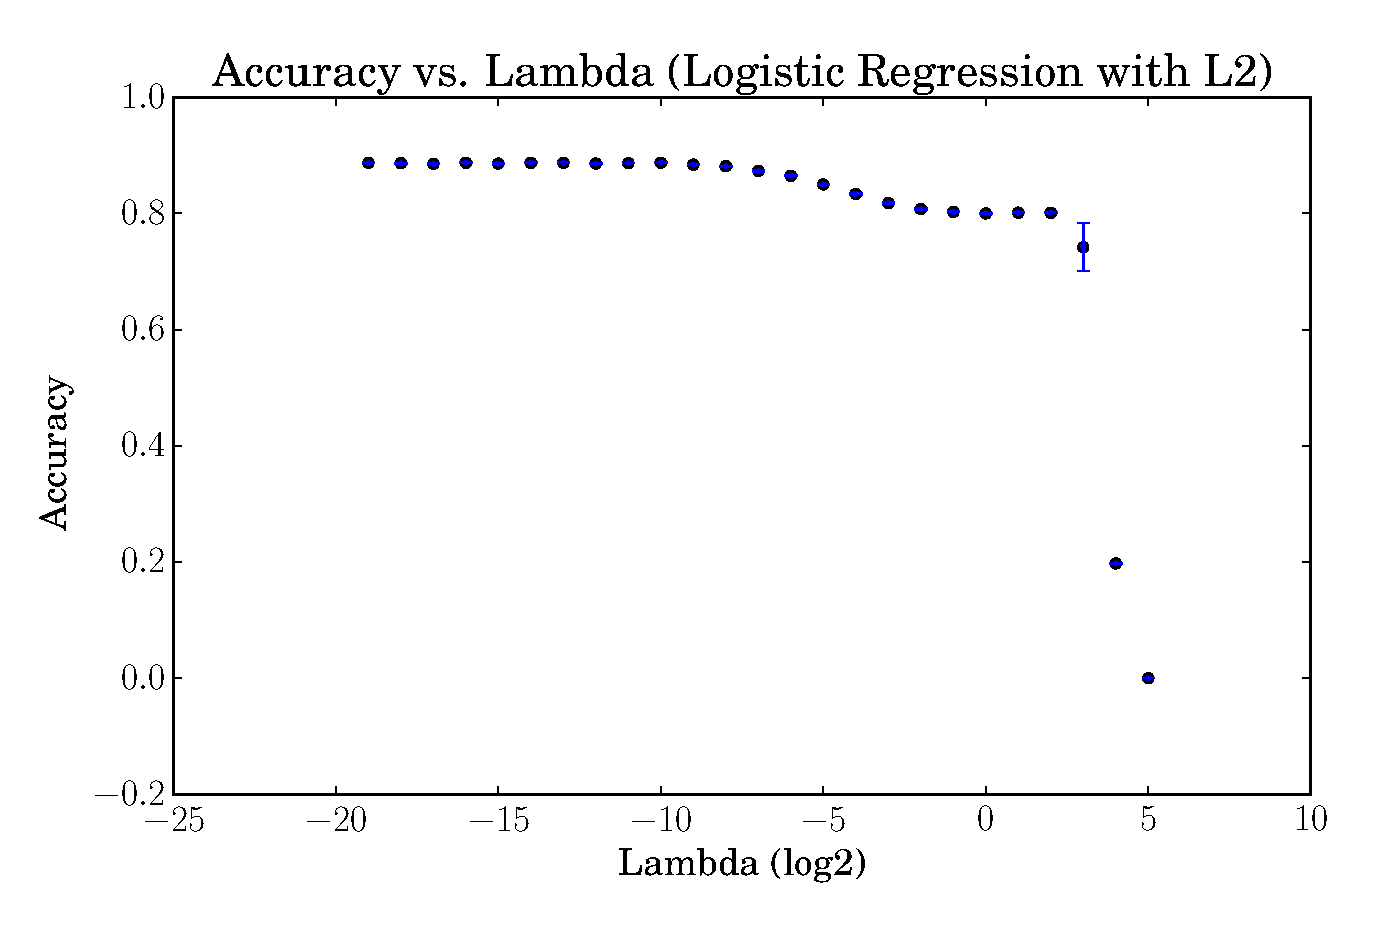
\includegraphics[width=\textwidth]{acc_vs_lambda_logregL2}
        \caption{}
        \label{fig:lambda_logregL2}
    \end{subfigure}
    \caption{Acurácia vs. Parâmetro $\lambda$, com parâmetros fixos:
    $\sigma=0.003$, $\alpha=2.0$, $I=500$}\label{fig:lambda}
\end{figure}

\newpage
\subsection{Acurácia vs. Tamanho do \textit{Batch} para o \texttt{Scikit Learn}} \label{sec:acc_vs_batchSKL}

A acurácia dos algoritmos do \texttt{Scikit Learn} se beneficiou mais do
aumento de tamanho do \textit{batch}. Acredito que isso se deva ao fato de que
as minhas implementações ainda tinham acesso ao conjunto total de dados, e
escolhiam ao acaso quais exemplos comporiam o \textit{batch} a ser utilizado
numa dada iteração. Assim, as implementações desse trabalho se beneficiaram do
conjunto total de dados e também do benéficio de realizar operações em porções
menores de exemplos. O erro padrão das medições também foi maior para esses
algoritmos.

\begin{figure}[htpb]
    \centering
    \begin{subfigure}[htpb]{0.45\textwidth}
        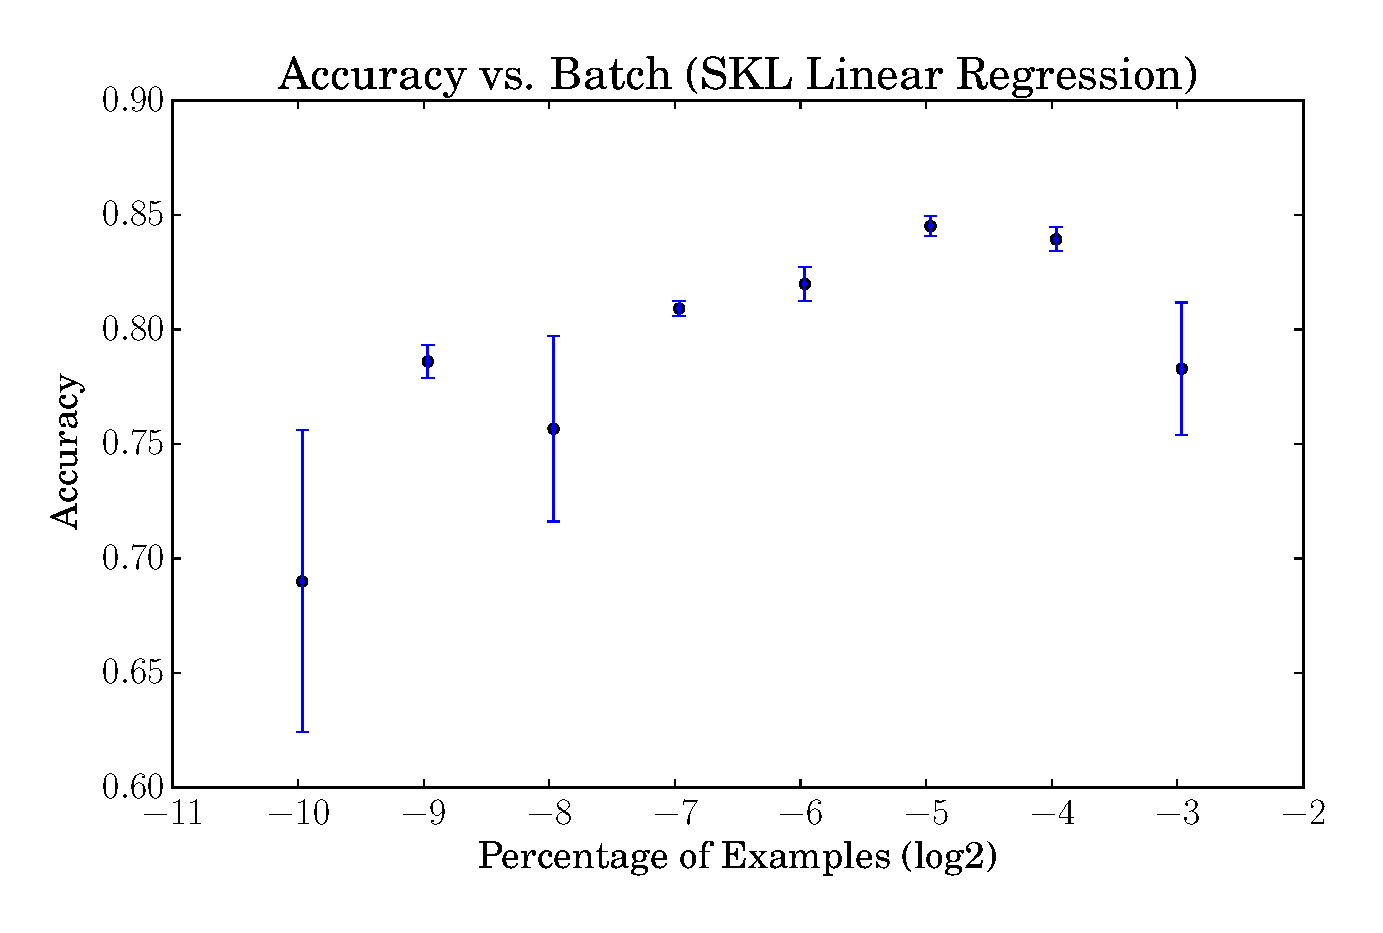
\includegraphics[width=\textwidth]{acc_vs_batchp_skl_linreg}
        \caption{}
        \label{fig:batch_skl_linreg}
    \end{subfigure}
    %add desired spacing between images, e. g. ~, \quad, \qquad, \hfill etc.
    %(or a blank line to force the subfigure onto a new line)
    \begin{subfigure}[htpb]{0.45\textwidth}
        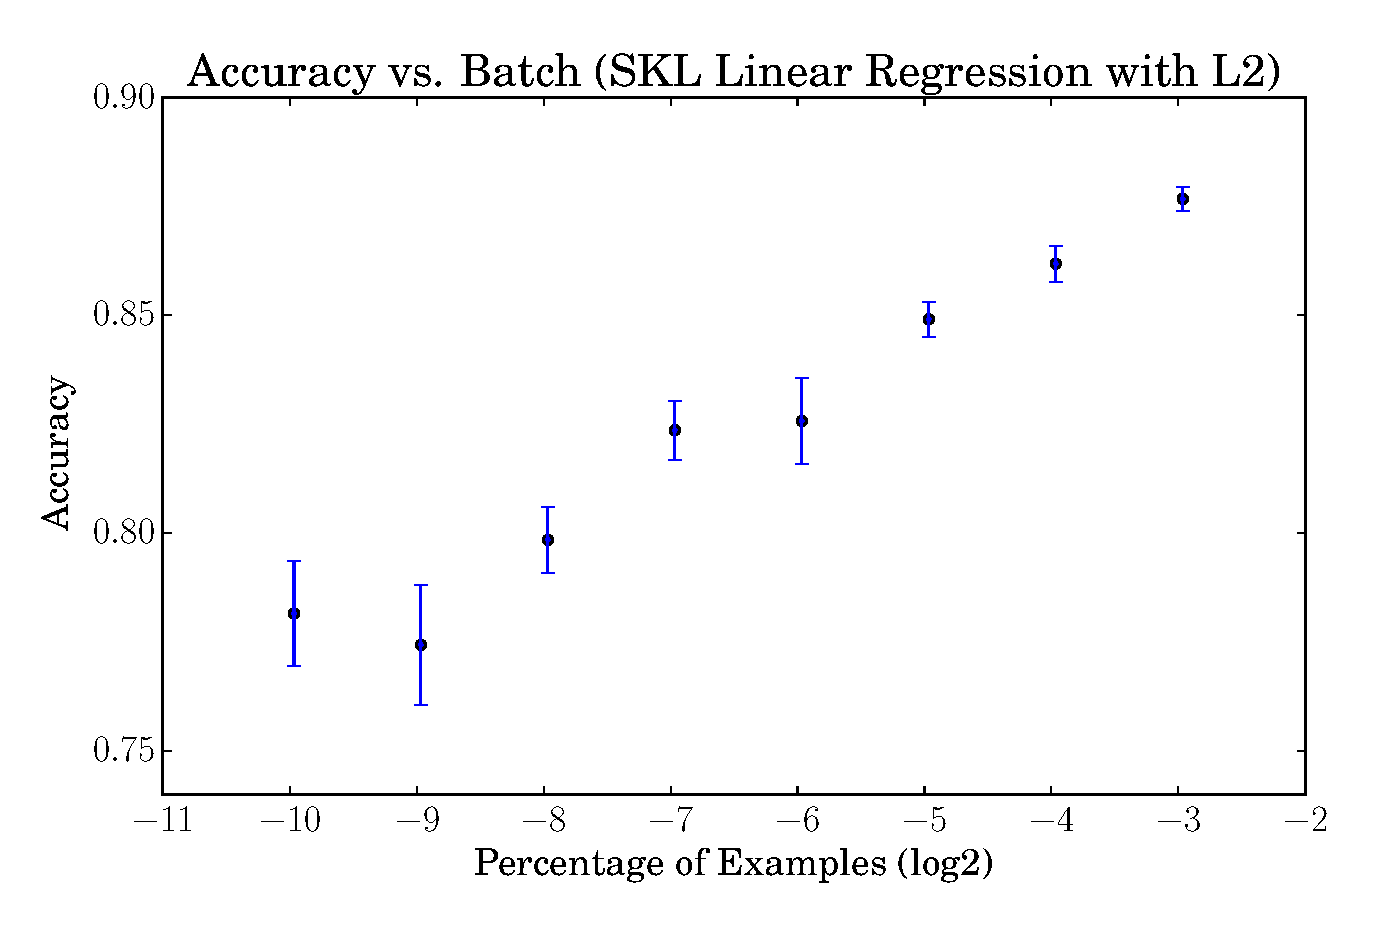
\includegraphics[width=\textwidth]{acc_vs_batchp_skl_linregL2}
        \caption{}
        \label{fig:batch_skl_linregL2}
    \end{subfigure}
    \hfill %add desired spacing between images, e. g. ~, \quad, \qquad, \hfill etc.
    %(or a blank line to force the subfigure onto a new line)
    \begin{subfigure}[htpb]{0.45\textwidth}
        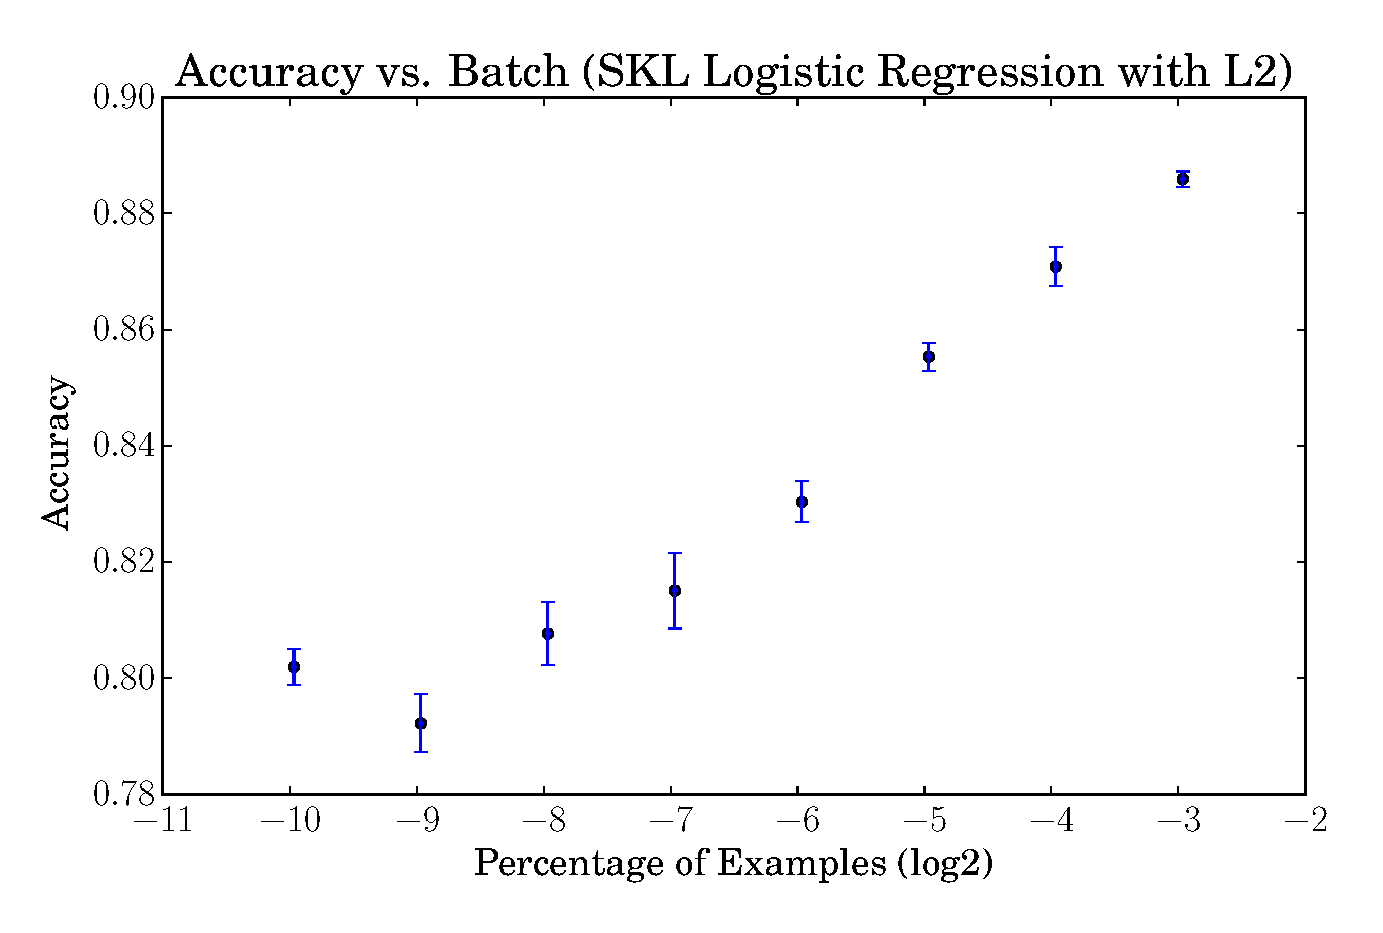
\includegraphics[width=\textwidth]{acc_vs_batchp_skl_logregL2}
        \caption{}
        \label{fig:batch_skl_logregL2}
    \end{subfigure}
    \caption{Acurácia vs. Tamanho do \textit{Batch} ($\sigma$)
    para algoritmos do \texttt{Scikit Learn}}\label{fig:batch_skl}
\end{figure}

\newpage
\subsection{Otimização dos Parâmetros}

A Tabela \ref{tab:par} apresenta a escolha de parâmetros para cada modelo feita
após os experimentos.  Como tanto a acurácia dos modelos como o tempo de
execução aumentam proporcionalmente ao número de iterações $I$ e ao tamanho do
\textit{batch} $\sigma$, escolhi os maiores valores possíveis desses
parâmetros, isto é, valores grandes o suficiente para uma boa acurácia, mas
com tempo de execução razoável.

\begin{table}[htpb]
    \centering
    \begin{tabular}{@{}lcc@{}}
        \textbf{Modelos} & \multicolumn{2}{c}{\textbf{Parâmetros}} \\ \toprule
        & $\lambda$ & $\alpha$ \\ \midrule
        Regr. Lin. & - & $0.25$ \\
        Regr. Log. & - & $2$ \\
        Regr. Lin. ($L_2$) & $2^{-4}$ & $0.25 $       \\
        Regr. Log. ($L_2$) & $2^{-10}$ & $0.5$ \\ \bottomrule
    \end{tabular}
    \caption{Escolha de parâmetros para as implementações, após os
    experimentos. Todos os modelos usaram o mesmo número de iterações,
    $I = 10^{4}$, e tamanho de \textit{batch}, $\sigma = 2^{-6}$ (aprox.
    $1.5\%$ do conjunto de dados por iteração)}
    \label{tab:par}
\end{table}

\newpage
\subsection{Comparação de Acurácia}

A Figura \ref{fig:algorithm} apresenta comparações da acurácia dos modelos
implementados neste trabalho e dos modelos disponíveis no \texttt{Scikit
Learn}, denotados por \lq\lq{}\textit{SKL}\rq\rq{} na figura.

Acredito que as minhas implementações tiveram acurácia maior que as
implementações do \texttt{Scikit Learn} por conta do motivo descrito na Seção
\ref{sec:acc_vs_batchSKL}: nas minhas implementações, o parâmetro $\sigma$
determina qual a \textit{porcentagem} do conjunto de exemplos que será
utilizada em cada iteração, mas não limita \textit{quais} exemplos podem ser
selecionados. A cada iteração, um novo conjunto de exemplos é selecionado. Nas
implementações do \texttt{Scikit Learn} o parâmetro $\sigma$ determina a qual
porcentagem do conjunto de exemplos o algoritmo terá \textit{acesso}.

Portanto, não é correto dizer que as acurácias das implementações deste
trabalho são maiores do que as de suas implementações correspondentes no
\texttt{Scikit Learn}. Ademais, é interessante notar que as implementações do
\texttt{Scikit Learn} têm tempo de execução muito menor do que as
implementações deste trabalho.

\begin{figure}[htpb]
    \centering
    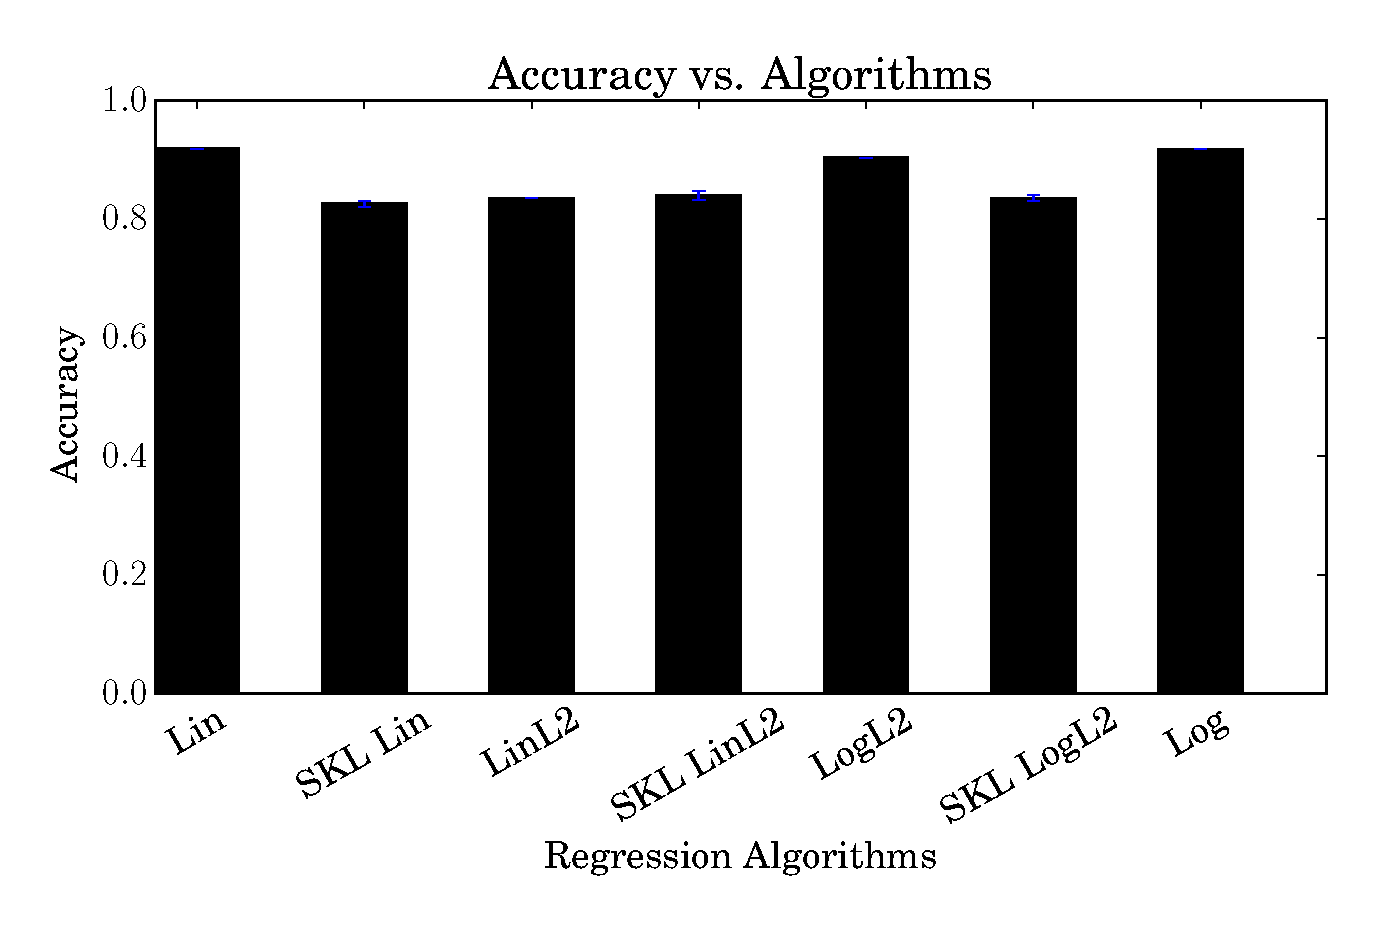
\includegraphics[width=.8\textwidth]{acc_vs_algorithm}
    \caption{Acurácia dos algoritmos implementados e do
    \texttt{Scikit Learn}. Os algoritmos foram executados
    com os parâmetros descritos na Tabela ~\ref{tab:par}}
    \label{fig:algorithm}
\end{figure}

\newpage
\section{Conclusão} \label{sec:concl}

Este relatório apresentou e discutiu implementações dos modelos de Regressão
Linear e Regressão Logística, usando o método de Regularização $L_2$. Foram
feitas análises de acurácia em relação à variação dos parâmetros mais
importantes desses modelos, e comparações de acurácia com implementações dos
modelos no pacote \texttt{Scikit Learn}.

\end{document}
